\documentclass[tikz,border=2pt]{standalone}
\usepackage{amsmath,amssymb}
\usepackage{tikz}
\usetikzlibrary{arrows.meta}

\begin{document}
% Rounding the LP optimum (3.5, 1.25): the nearest integer vector (4, 1) is infeasible, the
% feasible rounding (3, 1) is a candidate — never guaranteed to be optimal in general.
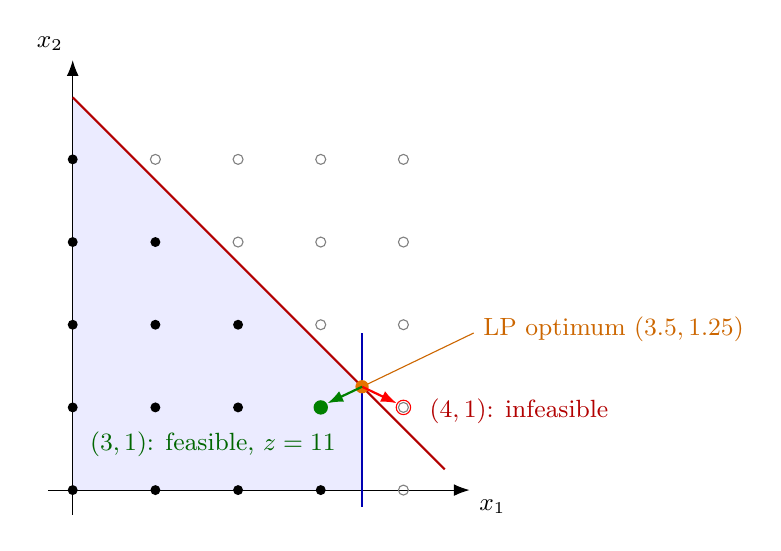
\begin{tikzpicture}[x=1.05cm, y=1.05cm, every node/.style={font=\small}, >={Latex[length=2mm]}]
	\fill[blue!8] (0,0) -- (3.5,0) -- (3.5,1.25) -- (0,4.75) -- cycle;
	\draw[->] (-0.3,0) -- (4.8,0) node[below right] {$x_1$};
	\draw[->] (0,-0.3) -- (0,5.2) node[above left] {$x_2$};
	\draw[blue!70!black, thick] (3.5,-0.2) -- (3.5,1.9);
	\draw[red!70!black, thick] (4.5,0.25) -- (0,4.75);
	\foreach \i in {0,1,2,3,4} {\foreach \j in {0,1,2,3,4} {
		\pgfmathparse{(2*\i+2*\j<=9.5 && \i<=3.5) ? 1 : 0}
		\ifnum\pgfmathresult=1 \fill[black] (\i,\j) circle (1.8pt); \else \draw[gray] (\i,\j) circle (1.8pt); \fi
	}}
	\draw[orange!80!black, thin] (3.5,1.25) -- (4.85,1.9);
	\fill[orange!90!black] (3.5,1.25) circle (2.4pt);
	\node[orange!80!black, font=\small, anchor=west] at (4.85,1.95) {LP optimum $(3.5,1.25)$};
	\draw[->, red, thick] (3.5,1.25) -- (3.92,1.05);
	\draw[red] (4,1) circle (2.6pt);
	\node[red!70!black, font=\small, anchor=west] at (4.2,0.95) {$(4,1)$: infeasible};
	\draw[->, green!50!black, thick] (3.5,1.25) -- (3.08,1.05);
	\fill[green!50!black] (3,1) circle (2.6pt);
	\node[green!40!black, font=\small, anchor=north east] at (3.3,0.82) {$(3,1)$: feasible, $z=11$};
	\end{tikzpicture}
\end{document}
